\documentclass{article}

\usepackage[utf8]{inputenc} %most IDEs use UTF8
\usepackage[T1]{fontenc} %most fonts needs T1
\usepackage{amsmath}
\usepackage{graphicx}

\begin{document}
\begin{titlepage}
    \begin{center}
        \vspace*{1cm}
        \Huge
        \textbf{A novel method to briefly localize the human movement on a flat surface}

        \vspace{1.5cm}


        \vspace{1.5cm}
        \LARGE
        \textbf{Zili Li}

        \vfill

        Script Not final version.

        \vspace{0.8cm}
        \normalsize

        National Engineering Research Center for E-Learning\\
        Central China Normal University\\
        China \\
        2024--06

    \end{center}
\end{titlepage}
\begin{abstract}
    This article propose a novel approach to localize human's movement on a flat surface using a fixed monocular camera. Assuming the person is moving on a flat surface and during the movement the person is not obscured by opaque objects.By solving a constrained perspective-3-point problem and filter the results using a modified Kalman filter.We can extract the localized movement information from the frames.
\end{abstract}
\section{Pinhole Camera Model} 
The pinhole camera model first introduced by Brunelleschi in the early fifteenth century provides a simple representation of how light interacts with a camera to form an image. The camera is represented as a simple opaque box with a tiny hole on one side and a flat plane on the opposite. All rays of light are blocked by the walls of the box except those passing through the tiny hole.
When an object is placed in front of the hole, rays of light reflecting or emitting from different points of the object pass through the hole to form an inverted image on the image plane. If Without the opaque box and the pinhole, every point on the plane would be illuminated from all points emitting or reflecting light from the object or the environment. Hence, the points on the image plane will be illuminated uniformly and no image can be observed.

\begin{figure}[h!]
    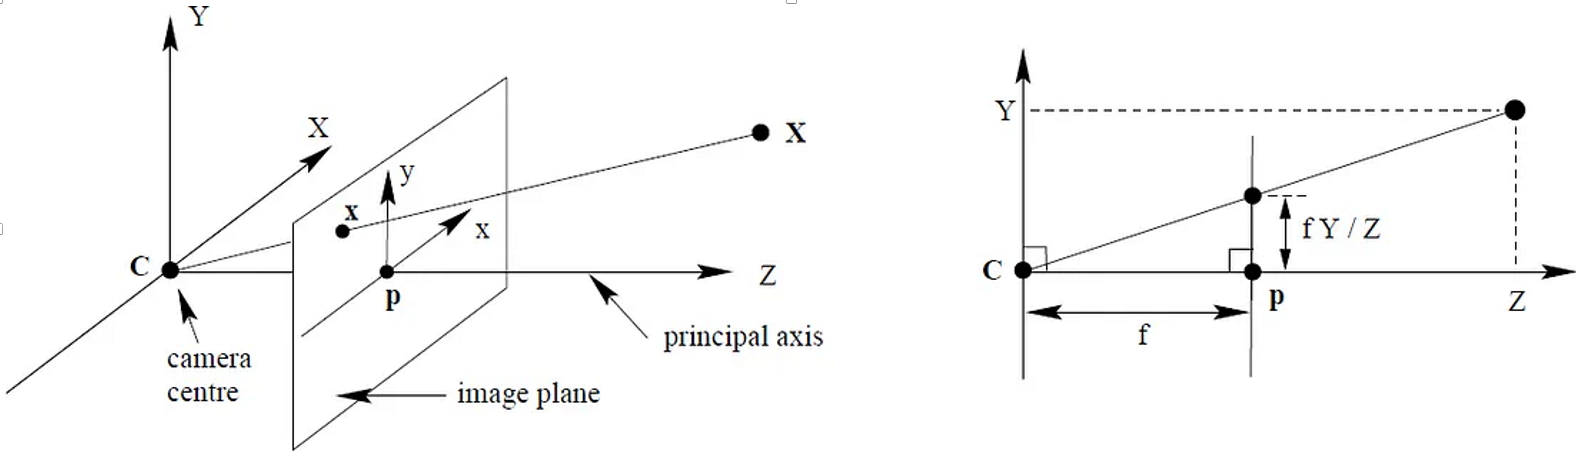
\includegraphics[width=\linewidth]{fig1.1.png}
    \caption{The pinhole camera model}\label{fig:1.1}
\end{figure}

The fig1.\ref{fig:1.1} represents the operating principle of the pinhole camera.

Objects farther away from the camera appear smaller in the image. The distance from the small hole to the image plane determines the field of view of the camera. A closer distance to image plane results in a smaller field of view, capturing more of the scene the image size of the distant object is proportional to the distance from the pinhole aperture to the image plane.

However, a real pinhole camera cannot work in most conditions since a small hole cannot let through enough light in an acceptable exposure time. Optical lens can gather much more light and however lens introduced optical distortions and aberrations to the image, making edge of the image sometimes unusable and corrections needed to restore properties of the image such as straight lines and color.

\section{The coordinate systems}
Here we must talk about the coordinates of the world coordinate and camera coordinates before we can give any meanful mathematical representations of out problem.

In the view of camera everything is pixels, and the camera locates pixels by camera coordinate $(u,v)$ (1) the origin of pixel is at upper left corner of the image and x goes to right y goes down.

In the 3-d world we can establish a coordinate system by using the camera as a reference.The origin locates at the focal point of the camera. We denote the coordinate as
 $(X_c,Y_c,Z_c)$ 
 and since world coordinate's origin locates at the focal point share $z$ axis with the camera. We can immediately have a 2D coordinate system which the $x,y$ axis is paraell to the $X_c Y_c$ and it's origin is at the principle point of the optical system on the image plane, for the analysis of the optical projection.
In the view of other stuff in the world, it has it's own coordinate and their own axis. We denote the coordinate as $(X,Y,Z)$.
\section{Camera Parameters}
\subsection[short]{The camera matrix}

The parameters of the camera intrinsic matrix are estimated by performing the camera calibration procedure. In our case the intrinsic matrix is obtained by manufactor of the camera.

The differences between different cameras can be described in these quantities:  

1. The focal length: The distance between the center of the projection and the image plane.

2. The center of projection: The point where the pinhole aperture is located against the image plane.

3. The optical axis is the line perpendicular to the image plane and passing through the center of projection.

4. The principal point is defined as the point of intersection between the optical axis and the image plane.

The focal length together with the sensor size determines the field of view and the magnification of the camera. A longer focal length results in a narrower field of view and magnifies distant objects, while a shorter focal length captures a wider field of view but diminishes the magnification of distant objects. Sensor size is the inverse of the focal length. Larger sensor is the same as we get shorter focal length smaller sensor is the same as we get longer focal length. We cannot determine the focal length just by measuring the size of items in the image.But for a known size of sensor it is possible.

The relation between a point \begin{equation}
    Q=(X_c, Y_c, Z_c)
\end{equation}in space under camera coordinate and its projection on the image plane under the 2D camera coordinate is \begin{equation}
    (x_s, y_s)
\end{equation} is represented by the following equations:
\begin{eqnarray}
    x_s=f_x\frac{X}{Z}+c_x \\
    y_s=f_y\frac{Y}{Z}+c_y
\end{eqnarray}

where $c_x$and $c_y$
are two parameters that handle possible misalignment of the principal point with the center of the image; $f_x$ and $f_y$
are essentially the focal lengths expressed in pixels. We introduce two new parameters because each pixel on a typical image plane is rectangular, hence the pixel lengths in x and y are different. It is worth noting that $x_s,y_s,c_x,c_y,f_x,f_y$are expressed in units of pixels.The physical focal length f, usually expressed in units of millimeters, cannot be measured directly. However, the focal lengths $f_x$ and $f_y$ can be measured using a procedure called camera calibration.
4. Camera Intrinsic Matrix
Projective transform is the function that maps the points in the space with coordinates$(X, Y, Z)$ to its projection $(x_s, y_s)$ on the image plane. It is customary to express such transform using the homogeneous coordinates, hence the equations above can be written to matrix form.
$M$ is a $3\times3$ matrix called camera intrinsic matrix:where $q$ and $Q$ are the coordinates of the projection coordinates  and the corresponding point in the space.Hence we can formulate the camera matrix:
\begin{equation}
    M = \begin{bmatrix}
        f_x&0&c_x \\
        0&f_y&c_y \\
        0&0&1
    \end{bmatrix}
\end{equation} 

The camera intrinsic matrix represents the internal parameters of a camera, including the focal length, and it allows to project 3D points in the world onto the 2D image plane.


\begin{align*}
    (X_w,Y_w,Z_w)\rightarrow Rigid Body translation &= (X_c,Y_c,Z_c)
    \\(X_c,Y_c,Z_c)\rightarrow Perspective projection &= (x,y)\\(x,y)\rightarrow camera correction &= (u,v)
\end{align*}
The corresponding matrix expression of the translations above
\begin{align}
    \begin{bmatrix}
        R_{3\times3} & T_{3\times1} \\O & 1
    \end{bmatrix}\begin{bmatrix}
                     X_w \\ Y_w \\ Z_w
                 \end{bmatrix} & = \begin{bmatrix}
                                       X_c \\ Y_c \\ Z_c
                                   \end{bmatrix} \rightarrow \\\begin{bmatrix}
        f_x & 0   & 0 & 0 \\
        0   & f_y & 0 & 0 \\
        0   & 0   & 1 & 0
    \end{bmatrix}\begin{bmatrix}
        X_c \\Y_c\\Z_c\\1
    \end{bmatrix}&= \begin{bmatrix}
        x \\y\\0\\1
    \end{bmatrix} \rightarrow\\
    \begin{bmatrix}
        scale_x & 0       & C_x \\
        0       & scale_y & C_Y \\
        0       & 0       & 1
    \end{bmatrix}\begin{bmatrix}
        x\\y\\1        
    \end{bmatrix} &=\begin{bmatrix}
        u\\v\\1
    \end{bmatrix}  
\end{align}


\section{Solving constrained perspective 3 points problem}
\subsection*{Problem formulation}

Given frame of a known camera calibrated for distortions, three 3D points $\boldsymbol{x_i}= (x_i,y_i,z_i)$, and corresponding homogeneous image coordinates $\boldsymbol{y_i} \in (u_i,v_i,1)$ and normalsize it s.t $|\boldsymbol{y_i}|= 1$, then:
 \begin{equation}
    \boldsymbol{\lambda_i} \boldsymbol{y_i} = \boldsymbol{R}\boldsymbol{x_i} +\boldsymbol{t}, i \in {1,2,3}
 \end{equation}
 where the rotation $\boldsymbol{R} \in SO(3)$ together with the translation $\boldsymbol{t} \in IR3$ define the pose of
 the camera. In short a P3P solver is a function $[\boldsymbol{R_k,t_k}] = P3P(x1:3,y1:3)$. Depending
 on the configuration of the points, P3P has up to four solutions.
 A necessary condition to assure the solutions are finate, is neither the 3D points nor the 2D points are collinear. In that case no information will be obtained on image plane. The solutions should be real numbers corresponding to coordinates. And the parameters $\lambda_k$ is the signed distance from the camera center for each 3D point, $\lambda_1,\lambda_2, $and $\lambda_3$ are required to be positive and real. This is a geometric feasibility condition on the solutions, which implies that all three 3D points are in the view the camera. Since we are working for a solution on a flat surface, we can filter out solution to further away from the surface.
 
\end{document}

